\documentclass[12pt]{article}

% packages :
\usepackage[utf8x]{inputenc}
\usepackage[T1]{fontenc}
%\usepackage[francais]{babel}
%
\usepackage{graphicx} % images
\usepackage{float}
\usepackage{placeins}
\usepackage{multirow}
\usepackage{wrapfig}
\usepackage{array}

% to draw circuits
\usepackage{siunitx}
\usepackage{tikz}
\usetikzlibrary{calc}
\usetikzlibrary{decorations.pathmorphing,patterns}

\usepackage[top=2cm, bottom=2cm, left=2.5cm, right=2.5cm]{geometry}


% maths :
\usepackage{amsthm}
\usepackage{amsmath}
\usepackage{amssymb}
\usepackage{mathrsfs}

\usepackage{braket}

\begin{document}

\begin{center}
    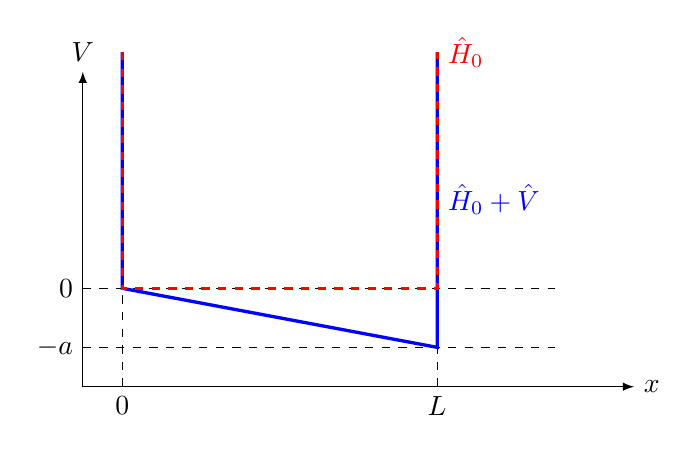
\begin{tikzpicture}
    \draw[-latex] (0,-.25) -- +(7,0) node[right]{$x$} ;
    \draw[-latex] (0,-.25) -- +(0, 4) node[above]{$V$};
    \draw[dashed] (.5,-.25) node[below]{$0$}-- +(0,3.5);
    \draw[dashed] (4.5,-.25) node[below]{$L$}-- +(0,3.5);
    \draw[dashed] (0,1)  node[left]{$0$} -- +(6,0);
    \draw[dashed] (0,.25)  node[left]{$-a$} -- +(6,0);
    
    \draw[very thick,blue] (.5,4) -- ++(0,-3) -- ++(4,-.75)  -- ++(0,3.75) node[midway,right]{$\hat{H}_0 + \hat{V}$};
    \draw[red,very thick,dashed] (.5,4) -- ++(0,-3) -- ++(4,0) -- ++(0,3) node[right]{$\hat{H}_0$};
    \end{tikzpicture}
\end{center}

\end{document}
